\vspace{-5pt}
\subsection{Background}

\noindent{\bf Error Correction and Evaluation} 

The majority of error correction tools share the following intuition: high-fidelity sequences (or, solid sequences) can be used to correct errors in low-fidelity sequences (or, in-solid sequences). However, they vary significantly in the way they differentiate between solid and in-solid sequences. For example, \cite{yang2010reptile} corrects genomic reads containing insolid $k$-mers using a minimum number of edit operations such that these reads contain only solid $k$-mers after correction.
% SB (1/28/18): Give some representative examples here (1-2 sentences). 
% Mustafa(1/28): done
The evaluation of \textit{de novo} sequencing techniques rely on likelihood-based metrics such as ALE and CGAL, without relying on the availability of a reference genome. On the other hand, comparative sequencing or re-sequencing, such as to study structural variations among two genomes, do have reference genomes available. 
% Moreover, the evaluation criteria for error correction techniques also vary based on the availability of a reference genome. For example, metrics such as Sensitivity, Specificity, and Gain, rely on a comparison with the reference genome to estimate the quality of the reads after correction. However, such metrics cannot be used for re-sequencing, where no reference genome is available, or when studying structural variations in known species. This is where \textit{Athena} whereby the use of the modeling perplexity metric removes the need for a reference genome.
% SB (1/28/18): And we do not have this problem. So mention that here. 
% SC (01/28): done

\noindent{\bf Language Modeling}

To increase the accuracy of detecting words in speech recognition, language modeling techniques have been used to see which word combinations have higher likelihood of occurrence than others, thus improving context-based semantics. Thus, language modeling is being used in many applications such as speech recognition, text retrieval, and many NLP applications. The main task of these statistical models is to capture historical information and predict the future sequences based on that information.
% Language models were originally targeted to improve the performance of automated speech recognition systems. However, they also play a critical role in a wide range of NLP problems. 

\noindent{\bf N-Gram-Based Language Modeling}. 
This type of modeling is word-based.
% , which means that each read has to be divided into several segments before we train such a model.
The main task that N-Gram based models \cite{brown1992class} have been used for is to estimate the likelihood of observing a word \textit{$W_i$}, given the set of previous words ${W_0, \cdots W_{i-1}}$, estimated using the following equation:
\newline
\begin{equation}
\begin{aligned}
  P(W_0, W_1, ..., W_{m}) &= \prod_{i=1}^{m}  P(W_{i} |  W_{i-1}, ..., W_{1}) \\
  &\approx \prod_{i=1}^{m}  P(W_{i} |  W_{i-1}, ..., W_{i-n})
  \end{aligned}
\end{equation}
\begin{figure}
  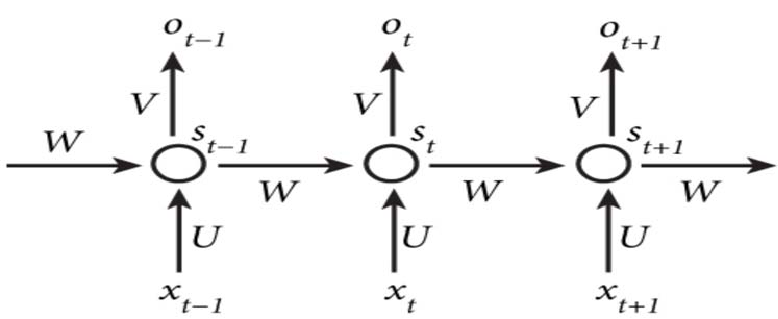
\includegraphics[width=0.9\linewidth]{figs/Background_RNN}
  \caption{Structure of a Recurrent Neural Network consisting of a chain of repeating modules of neural networks. The RNN predicts the next character at each time step $(t+1)$, knowing the history of characters in previous time steps.}
\label{fig:RNN}
\end{figure}
Where \textit{n} represents the number of history words the model uses to predict the next word. Obviously, a higher $n$ results in better prediction, at the cost of higher training time resulting from a more complex model.  

\noindent{\bf Char-RNN-Based Language Modeling}.
Recurrent neural network (RNN) is a very popular class of neural networks for dealing with sequential data, frequently encountered in the NLP domain. The power of RNN is that each neuron or unit can use its internal state memory to save information from the previous input and use that state, together with the current input, to determine what the next output should be. %In this context, we utilize this property to capture long character sequences and relations such as Genome Sequencing with similar way of Language modeling problems in machine learning applications.
Character-level RNN models, \textit{char-RNN} for short, operate by taking a chunk of text and modeling the probability distribution of the next character in the sequence, given a sequence of previous characters. This then allows it to generate new text, one character at a time~\cite{graves2013generating}.
As shown in Fig. \ref{fig:RNN}, RNNs consist of three main layers: Input Layer, Hidden Layer, and Output Layer.
First, Input Layer takes $ x_{t} $ vector, which is input at a time step $t$, usually a one-hot encoding vector of the $ t^{th} $ word or character of the input sentence. 
Second, Hidden Layer consists of the hidden state at the same time step $ s_{t} $, which represents the memory of this network. It is calculated as a non-linear function \textit{f} (\eg tanh ) of the previous hidden state $ s_{t-1} $ and the input at current time step $ x_{t} $ with the following relation: \begin{equation}
s_{t} = f(U x_{t} + W s_{t-1}).
\end{equation}
where, $W$ is a matrix that consists of hidden weights of this hidden layer.
Finally, Output Layer consists of a vector $ o_{t} $, which represents the output at step $t$ and contains prediction probabilities for the next character in the sentence. Formally, its length equals the size of the vocabulary and is calculated using a softmax function.
%\begin{equation}\label{eq:3}
%o_{t} = \mathrm{softmax}(V s_t).
%\end{equation}
% SB (1/28/18): The above equation is a CFC (Candidate For Chop). Softmax is just one of several possibilities. Plus we do not really use this equation in our text later. 
% Mustafa(1/28): done
Backpropagation was used to train the RNN to update weights and minimize the error between the observed and the estimated next word. For Deep RNN architectures, there are multiple parameters that affect the performance of the model. The two main parameters are: \textit{Number of Hidden Layers} and \textit{Number of Neurons per Layer}. For Char-RNN language modeling, vocabulary would include the four nucleotide bases as characters {A, C, G, and T}. Each input is a one-hot encoding vector for the four nucleotides.
% SB (1/28/18): Do we mean ``Each input is a one-hot encoding vector ...''. 
% Mustafa(1/28): done
Each output vector at each time step also has the same dimension.  

\noindent{\bf Perplexity of the Language Model}. 
Perplexity is a measurement of how well a probability distribution predicts a sample. In NLP, perplexity is one of the most effective ways of evaluating the goodness of fit of a language model since a language model is a probability distribution over entire sentences of text~\cite{azzopardi2003investigating}. For example, 5 per word perplexity of a model translates to the model being as confused on test data as if it had to select uniformly and independently from 5 possibilities for each word. Thus, a lower perplexity indicates that language model is better at making predictions.
For an N-Gram language model, perplexity of a sentence is the inverse probability of
the test set, normalized by the number of words. It is clear from \eqref{eq:4} that minimizing perplexity is the same as maximizing the probability of the observed set of $m$ words from $W_{1}$ to $W_{m}$.

\begin{equation}\label{eq:4}
\begin{aligned}
PP(W) &= \sqrt[m]{\frac{1}{P(W_{1},W_{2},....,W_{m})}}\\
&\approx \sqrt[m]{\frac{1}{\displaystyle \prod_{i=1}^{m}P(W_{i} | W_{i-1},...,W_{i-n})}}
\end{aligned}
\end{equation}
For RNN, perplexity is measured as the exponential of the mean of the cross-entropy loss (CE), given by:
\begin{equation}
\begin{aligned}
CE(y, \hat{y}) = - \sum_{i=1}^{|V|} y_{i}\log(\hat{y_i}),
\end{aligned}
\end{equation}
Where $\hat{y}$ is the predicted next character, the output of the RNN, and $|V|$ is the vocabulary size used during training. 
